\newpage
\section{Введение}

	\subsection{Некоторые определения}

	\begin{figure}[ht]
		\centering
		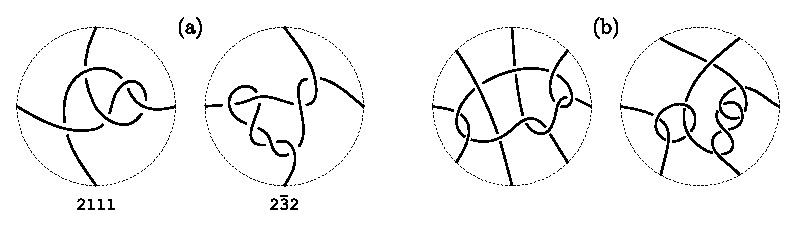
\includegraphics{c/tangles-example.eps}
		\caption{$2$-танглы (a), $k$-танглы в общем случае (b)\label{figure:tangles-example}}
	\end{figure}

	\begin{definition}
		\label{definition:tangle}
		$k$-танглом называется гладкое вложение $k$ отрезков и конечного числа окружностей в $B^3$
		(трехмерный замкнутый шар единичного радиуса), если $2k$ концов отрезков взаимно однозначно отображаются
		на точки с координатами $(\cos\pi i/k, \sin\pi i/k, 0)$, $i\in\{0, 1, \dots, 2k{-}1\}$, называемые
		концами $k$-тангла, и больше ни какие точки отрезков или окружностей на границу $B^3$ не отображаются.
	\end{definition}

	\begin{definition}
		\label{definition:tangle-equiv}
		$k$-танглы $T_1$ и $T_2$ называются эквивалентными, если существует изотопия $B^3$, сохраняющая границу
		неподвижной, которая переводит $T_1$ в $T_2$.
	\end{definition}

	\begin{definition}
		$k$-танглы $T_1$ и $T_2$ называются слабо эквивалентными, если существует изотопия $B^3$ (не обязательно
		сохраняющая границу неподвижной) которая переводит $T_1$ в $T_2$.
	\end{definition}

	\begin{figure}[ht]
		\centering
		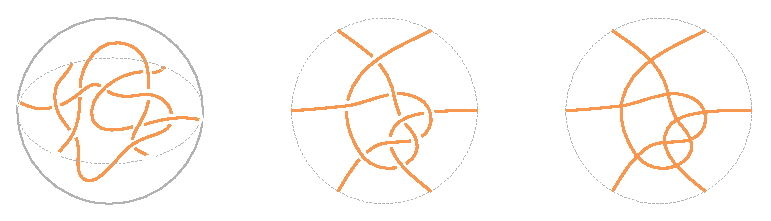
\includegraphics{c/tangle-diagram-projection.eps}
		\caption{$3$-тангл, его диаграмма и проекция\label{figure:3-tangle-and-proj}}
	\end{figure}

	Аналогично узлам и зацеплениям мы можем ввести понятие диаграммы и для $k$-танглов, строя невырожденные проекции
	$k$-тангла на плоскость, проходящую через его концы. Из \figureref{figure:tangles-example} \figureref{figure:3-tangle-and-proj}
	можно получить интуитивное представление о том, что такое диаграммы; строгое определение и подробное обсуждение
	``тонких мест'', напрямую не относящихся к нашей текущей теме, читатель может найти, например, в книге \cite{Cromwell2004}.
	Диаграммы, которые отличаются только плоской изотопией, сохраняющей граничную окружность, мы различать не будем.

	\begin{definition}
		Перекрестками диаграммы (проекции) называются точки, в которые проецируются две точки $k$-тангла. Ребрами
		диаграммы (проекции) называются максимальные множества точек, не лежащие на границе, в которые проецируется
		только по одной точке $k$-тангла.
	\end{definition}

	Ребра гомеоморфны открытым отрезкам и соединяют либо 2 перекрестка, либо 2 конца $k$-тангла либо конец с перекрестком.

	\begin{definition}
		Минимальной диаграммой $k$-тангла $T$ называют диаграмму $T$ с минимальным количеством перекрестков.
	\end{definition}

	\begin{figure}[ht]
		\centering
		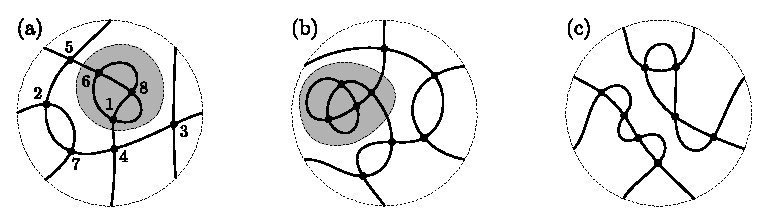
\includegraphics{c/composite-non-connected-projections.eps}
		\caption{Составные (a, b) и несвязные (c) проекции\label{figure:composite-proj}}
	\end{figure}

	\begin{definition}
		Диаграмма (проекция) $k$-тангла называется составной, если строго внутри граничной окружности существует замкнутая
		гладкая несамопересекающаяся кривая, которая трансверсально пересекает диаграмму ровно в двух точках и содержит
		внутри как минимум один перекресток. В противном случае диаграмма называется простой.
	\end{definition}

	\begin{definition}
		$k$-тангл называется простым, если просты все его минимальные диаграммы.
	\end{definition}

	\begin{definition}
		Диаграмма (проекция) называется связной, если граф, ребрами которого являются ребра диаграммы (проекции), а
		вершинами --- вершины и концы диаграммы (проекции), является связным.
	\end{definition}

	\begin{definition}
		$k$-тангл называется связным, если связна любая его диаграмма.
	\end{definition}

	\begin{definition}
		Диаграмма $k$-тангла называется альтернированной, если у каждого ребра, соединяющего два перекрестка, один из
		концов проходит над перекрестком, а другой --- под.
	\end{definition}

	\begin{definition}
		$k$-тангл называется альтернированным, если он имеет альтернированную диаграмму.
	\end{definition}


	\subsection{Постановка задачи}

	Как и в случае с узлами и зацеплениями, было бы логично поставить задачу классификации и для $k$-танглов. На настоящий
	момент результаты в этой области имеются в основном только для $2$-танглов. Общий случай уже интересен сам по себе,
	более того $k$-танглы могут оказаться полезными для исследованиях в других областях, например, для представления узлов
	и зацеплений в замкнутых ориентируемых поверхностях произвольного рода \cite{Kauffman1999, Kuperberg2003} --- так называемых
	виртуальных узлов и зацеплений.

	Так в работе \cite{Conway1970} J.~Conway ввел понятие танглов (которые в соответствии с Определением~\ref{definition:tangle}
	являются $2$-танглами) в качестве средства для описания и классификации узлов и зацеплений. Там же была предложено разделение
	танглов на классы рациональных, алгебраических и трансцендентных. Самым поддающимися исследованию оказались рациональные
	танглы --- для них проблема классификации была полностью решена \cite{KauffmanLambropoulou2004}.

	Для простых альтернированных $2$-танглов было получено полиномиальное уравнение на производящую функцию
	\cite{SundbergThistlethwaite1998}, которое затем было использовано там же для улучшения оценок на количество простых
	альтернированных зацеплений.

	Матричные интегралы рассматриваются как средство для перечисления альтернированных $k$-танглов в
	\cite{Justin1999_1, Justin1999_2, JustinZuber2000, Justin2001, JacobsenJustin2002, JustinZuber2003}.
	Там приведены теоретические результаты,	а также численно полученная таблица количеств простых альтернированных 
	$2$- и $3$-танглов. Однако сложность предложенного метода быстро растет с увеличением $k$.

	Наконец в \cite{KanenobuSaitoSatoh2003} с точностью до слабой эквивалентности были классифицированы простые $2$-танглы
	не более, чем с семью перекрестками.

	Целью данной работы является алгоритм, позволяющий получить все альтернированные $k$-танглы (а точнее их минимальные диаграммы)
	с количеством перекрестков, не превосходящим заданное число. Иными словами проделать то же самое для альтернированных танглов,
	что было сделано в \cite{Rankin2002_1, Rankin2002_2, Rankin2002_3} для альтернированных зацеплений. Однако, класс рассматриваемых
	$k$-танглов стоит ограничить уже по той причине, что всего их, даже с конечным числом перекрестков, бесконечное число. Поэтому
	мы будем рассматривать только связные альтернированные танглы. Также из рассмотрения традиционно исключаются составные
	диаграммы --- так мы и будем поступать.

	Выбор класса альтернированных $k$-танглов обусловлен рядом их известных свойств, сильно облегчающих задачу. В частности,
	любая минимальная диаграмма простого альтернированного тангла является альтернированной и, кроме того, все его минимальные диаграммы
	могут быть получены друг из друга применением (возможно, многократным) преобразования, называемого ``flype''
	(см. \figureref{figure:flype}). Также любая нередуцируемая (т. е. такая, в которой нельзя сразу же ``распутать'' петлю
	первым движением Редемейстера, тем самым уменьшив число перекрестков), в частности --- простая, альтернированная диаграмма
	является минимальной диаграммой.

	\begin{figure}[ht]
		\centering
		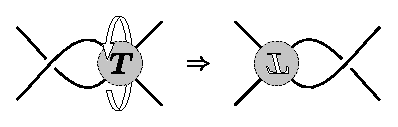
\includegraphics{c/flype.eps}
		\caption{Flype\label{figure:flype}}
	\end{figure}

	P.~G.~Tait более 100 лет назад \cite{Tait1900} выдвинул предположение о возможности получения минимальных альтернированных диаграмм
	узлов и зацеплений друг из друга с помошью преобразования \figureref{figure:flype}, получившее название ``Tait flyping conjecture''.
	Доказано оно было относительно недавно W.~Menasco и M.~Thistlethwaite в \cite{MenascoThistlethwaite1991, MenascoThistlethwaite1993},
	а утверждения выдвинутые выше являются являются его простыми обобщениями и следствиями.

	Как правило в литературе (в нашем случае это во всех ссылках, кроме \cite{KanenobuSaitoSatoh2003}) для перечисления танглов
	используются аналитические методы, поэтому там используется Определение~\ref{definition:tangle-equiv} для определения эквивалентности
	двух $k$-танглов, так как оно дает наиболее простые соотношения. Мы, однако, собираемся явно получать проекции всех простых связных
	альтернированных $k$-танглов с количеством перекрестков не превосходящим заданное число, значит заинтерисованы в максимальном сокращении
	количества ненужной работы. Поэтому имеет смысл отождествлять две диаграммы $k$-танглов, отличающиеся действием элемента
	группы $D_{2k}$ в дополнение к разрешенным Определением~\ref{definition:tangle-equiv} преобразованием. Очевидно, что большая часть
	танглов несимметрична, поэтому уже для $2$-танглов мы получаем выигрыш почти в 8 раз, а с ростом $k$ он становится все более
	значительным.

	Схема дальнейшей части работы выглядит следующим образом: в Главе~\ref{section:projections} мы рассмотрим алгоритм генерации
	всех возможных неэквивалентных (с точностью до плоской изотопии и $D_{2k}$) простых связных проекций $k$-танглов, затем мы
	покажем как модифицировать его для генерации простых альтернированных танглов в Главе~\ref{section:alternating}. Наконец,
	в Главе~\ref{section:drawing} приводится алгоритм создания ``красивых'' изображений $k$-танглов, который, конечно,
	непосредственного отношения к рассматриваемым вопросам не имеет, но является настолько полезным в процессе исследования, что
	фактически без него невозможно обойтись.
